\newpage
\addcontentsline{toc}{section}{OCLA Debug Subsystem}

\section*{ \hfill OCLA Debug Subsystem}


% \lipsum
\addcontentsline{toc}{subsection}{The Generated OCLA IP Wrapper}


\subsection*{\fontsize{14}{16}\selectfont The Generated OCLA IP Wrapper}
The IP customization and generation step is followed by the availability of a top wrapper and all source files for the user. The generated top wrapper file for the OCLA (see figure \ref{fig:ocla_wrpr}) comprises of two distinct clock domains, namely the sample clock and the AXI clock. 
\\ \\It is crucial to note that the sample clock of the OCLA should be connected to the design being monitored, while the AXI clock should be connected to the AXI bus clock.
\\ \\The signals of the design that are intended to be sampled are connected to the probes port of the OCLA. In addition, the user-specified optional input triggers signals can be connected to the corresponding port in the top wrapper.
\\ \\For configuring the OCLA and reading the sampled data from the system, the AXI-lite slave interface must be connected to an AXI bus.
% \begin{figure}[h]\centering % Using \begin{figure*} makes the figure take up the entire width of the page
% 	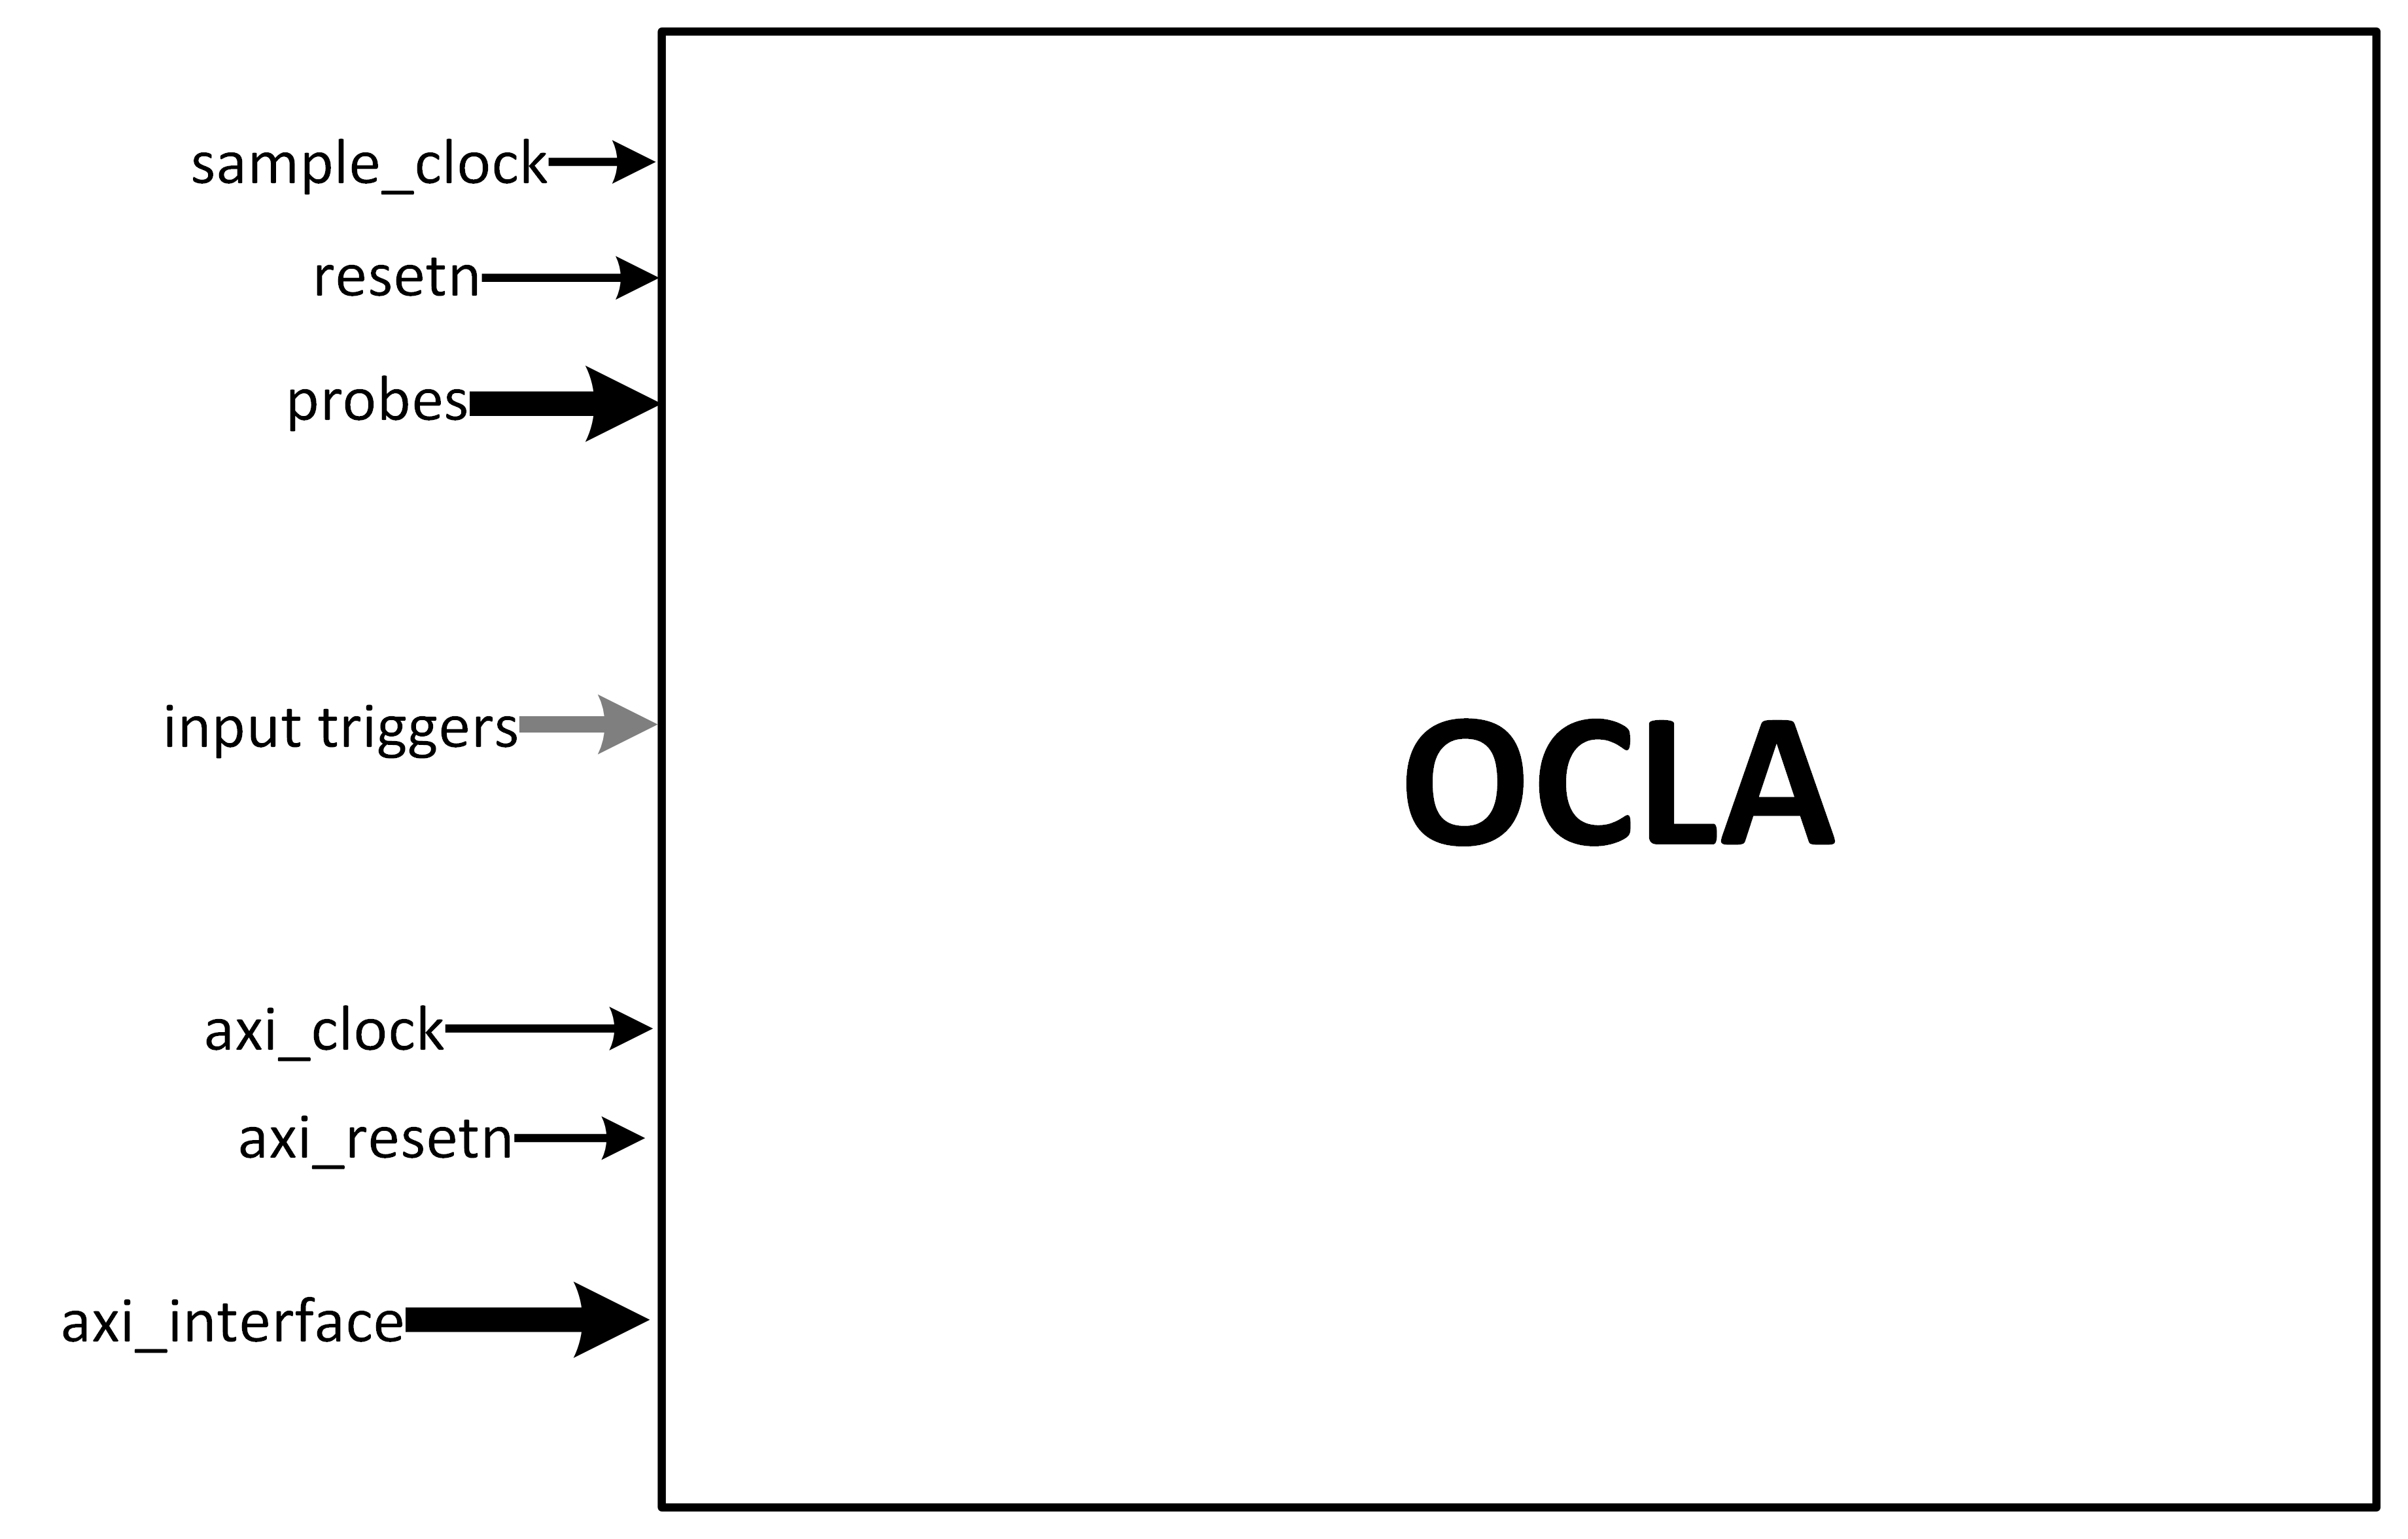
\includegraphics[width=.5\linewidth]{ocla_wrpr}
% 	\caption{\textbf{Figure \ref{fig:ocla_wrpr}.} OCLA TOP}
% 	\label{fig:ocla_wrpr}
% \end{figure}
% % \lipsum

\subsection*{\fontsize{14}{16}\selectfont OCLA Debug Subsystem}
\addcontentsline{toc}{subsection}{OCLA Debug Subsystem}
 The OCLA IP core, a component used for debugging purposes, can be instantiated within a subsystem. The debug subsystem, as depicted in Figure \ref{fig:ocla_subsystem}, integrates the OLCA IP core within the AXI bus and the design being monitored. The purpose of this integration is to allow for the runtime configurations of OCLA configurations through the use of the JTAG interface.
\\ \\This interface serves as the primary means of controlling and configuring the OCLA IP core within the subsystem, enabling the debugging process to proceed efficiently.
% \lipsum

\begin{figure}[h]\centering % Using \begin{figure*} makes the figure take up the entire width of the page
	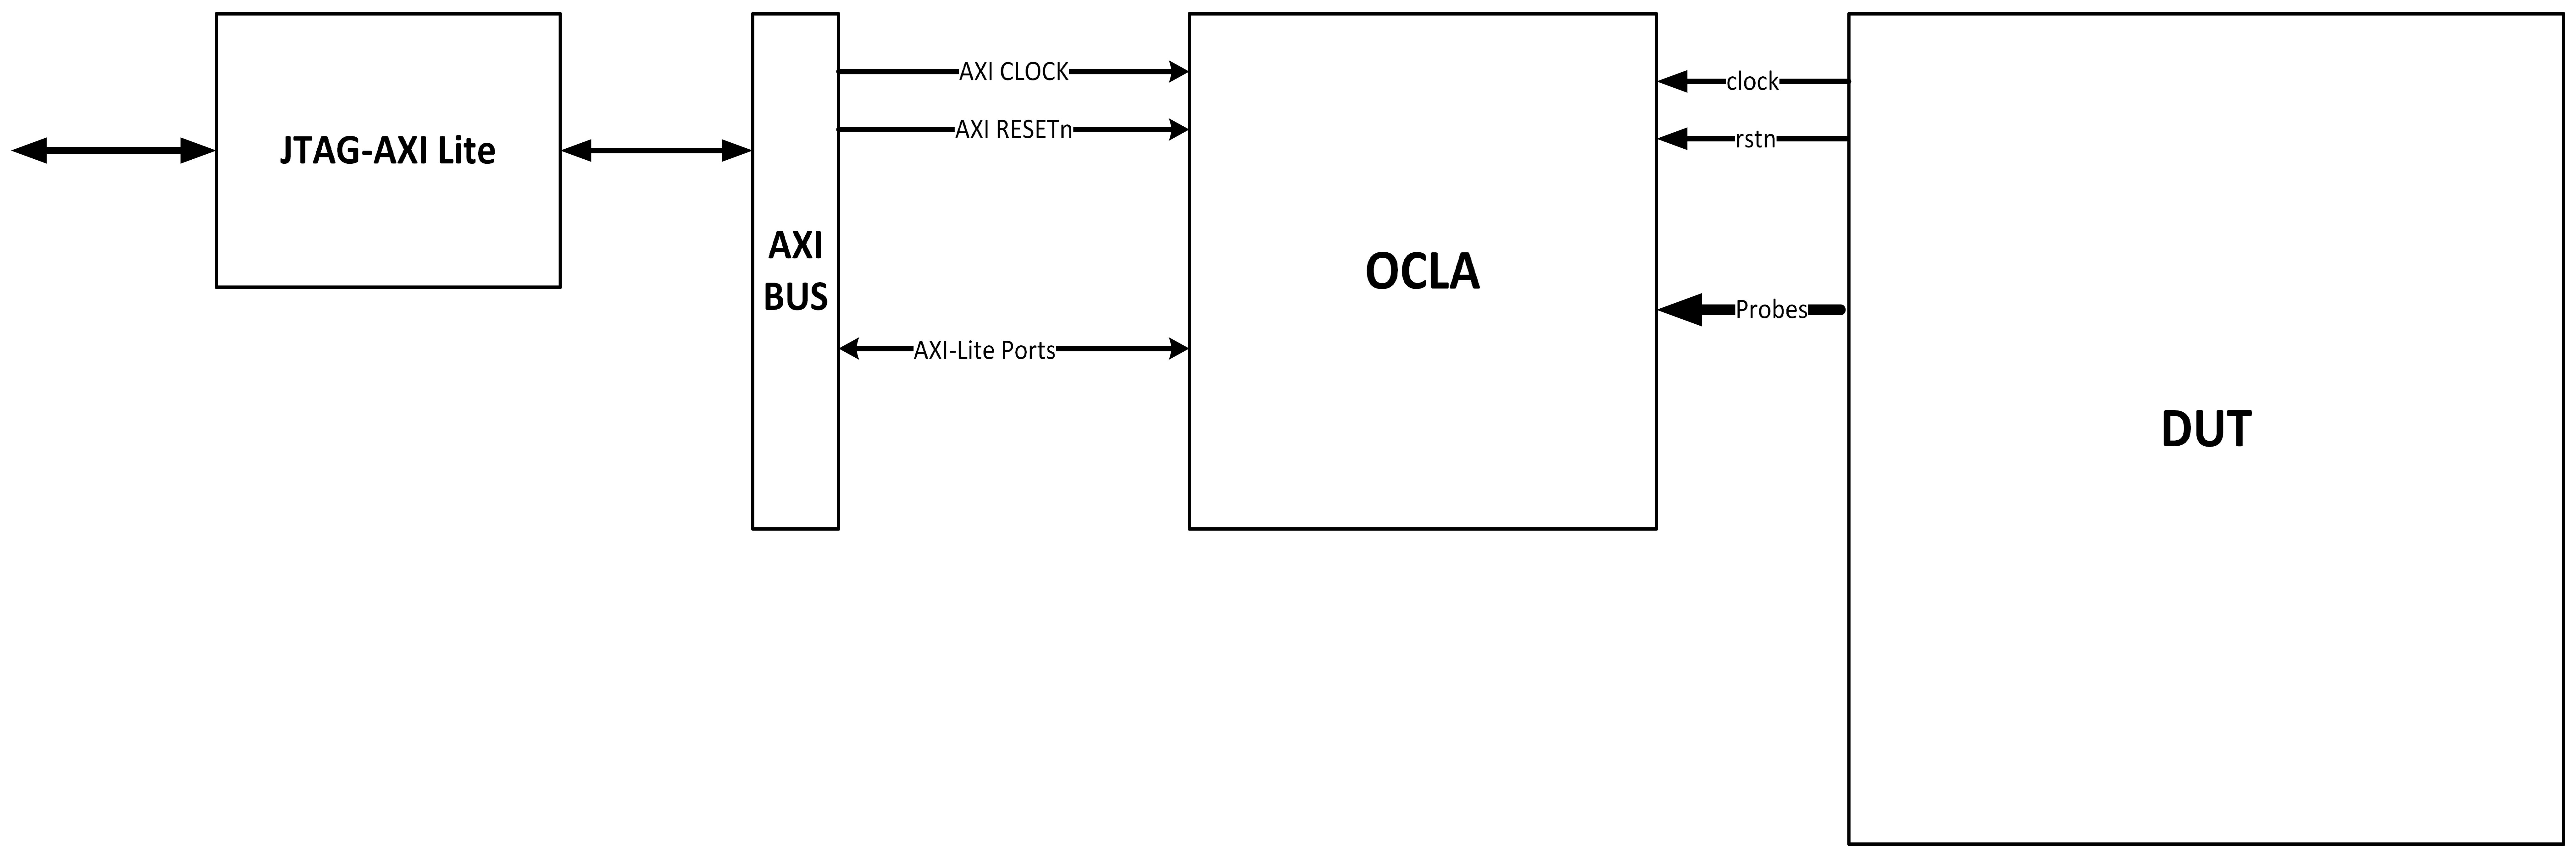
\includegraphics[width=\linewidth]{ocla_subsystem}
	\caption{\textbf{Figure \ref{fig:ocla_subsystem}.} OCLA Debug Subsystem}
	\label{fig:ocla_subsystem}
\end{figure}

% \lipsum

